\chapter{Literature Review}\label{chap:exres}

In this chapter, we will discuss the nature of existing threats to data, and the
ongoing research in this area.  We will then consider the specific threats posed
by e-mail.

\section{General Data Leakage}

The importance of data leakage is gaining more importance as the amount of
information stored about entities increases, and the risks are being considered
more carefully.  From the obvious ramifications for businesses discussed in
\cite{papadimitriou2011data}: the loss of trust and legal action resulting from
the discovery of leaking data, to the more personal issues discussed in
\cite{irani2011modeling}: the possibility of using the discovered data to
discover passwords or to physically identify them.  53\% of Americans can be
uniquely identified by their birthdate, gender and location (city/town), with
the number jumping 87\% when using birthdate, gender and zip code.

\subsection{Personal Data Leakage}

From a persona perspective, there are a number of risks.  There are a
significant number of social networks available, with an estimated 1.65 billion
monthly active users, with a significantly higher proportion used in developed
countries.  \cite{irani2011modeling} showed the rate at which the information
gathered from social networks can be used to uniquely identify anindividual,
with only 9 sites required before there's approximately a 70\% chance that both
a person's hometown and name could be recovered.  A similar number of sites can
give an aggregate normalised attribute leakage of 1, where the leakage is
defined as \[\Psi(F_a,P)=\frac{\sum_{f_a\in F_a}\phi\left(f_a,
			P\right)}{|F_a|}\text{ where }\phi\left(f_a, P\right) =
	\left[f_a\in P\right]\]

\subsection{Corporate Data Leakage}

When companies receive user data, they often have a legal obligation to ensure
that the data is protected and treated as confidential and sensitive.  When
this trust is broken, there are often severe consequences, both from regulators
and consumers moving their business to competitors.
\cite{squicciarini2010preventing} considers one way that data may be leaked,
despite care being taken to ensure that it is properly encrypted and stored. By
failing to protect against the indices for databases being stored insecurely,
customer data may be leaked.  Order-preserving encryption schemes, as decribed
in~\cite{agrawal2004order}, is one way of solving this problem, to an extent.

\section{Data Leakage from E-Mails}

\subsection{E-Mail Headers}

All e-mails include additional information about the sender and receiver, some
of which is used by an e-mail client in order to display more information about
the message that is currently being viewed, such as its original sender,
reply-to addresses and the time it was sent.  Additional fields allow senders to
authenticate themselves using public-key methods.

The format of e-mail headers was first defined in RFC~822, and further refined in
subsequent RFCs.  The standard for e-mails was then formalised precisely in
RFC~5322.

\subsection{Example Header and Pertinent Data}

In the example below, and text highlighted with red, \colorbox{red!30}{like
so} is information about the receiver.  Information about the sender, their
hardware or software is highlighted in green, \colorbox{green!30}{like so}; and
information gathered about intervening devices is highlighted in blue,
\colorbox{blue!30}{like so}.

\begin{lstlisting}
Delivered-To: |\colorbox{red!30}{joshuaclark94@gmail.com}|
Received: by |\colorbox{blue!30}{10.25.150.146}| with |\colorbox{blue!30}{SMTP}| id y140csp543137lfd;
	Sat, 6 Feb 2016 08:49:56 -0800 (PST)
X-Received: by |\colorbox{blue!30}{10.112.12.2}| with |\colorbox{blue!30}{SMTP}| id u2mr8302831lbb.145.1454777396580;
	Sat, 06 Feb 2016 08:49:56 -0800 (PST)
Return-Path: <agatabor@poczta.onet.pl>
Received: from |\colorbox{blue!30}{smtpo75.poczta.onet.pl}| (smtpo75.poczta.onet.pl. [|\colorbox{blue!30}{141.105.16.25}|])
	by mx.google.com with |\colorbox{blue!30}{ESMTPS}| id o199si12255636lfb.94.2016.02.06.08.49.56
	for <joshuaclark94@gmail.com>
	(version=TLS1_2 cipher=ECDHE-RSA-AES128-GCM-SHA256 bits=128/128);
	Sat, 06 Feb 2016 08:49:56 -0800 (PST)
Received-SPF: pass (google.com: domain of agatabor@poczta.onet.pl designates
		141.105.16.25 as permitted sender) client-ip=141.105.16.25;
Authentication-Results: mx.google.com;
spf=pass (google.com: domain of agatabor@poczta.onet.pl designates 141.105.16.25
		as permitted sender) smtp.mailfrom=agatabor@poczta.onet.pl
Received: from [10.26.196.156] (client-8-32.eduroam.oxuni.org.uk [|\colorbox{green!30}{192.76.8.32}|])
(Authenticated sender: |\colorbox{green!30}{agatabor@poczta.onet.pl}|)
by |\colorbox{blue!30}{smtp.poczta.onet.pl}| (Onet) with |\colorbox{blue!30}{ESMTPA}| id 3pyKNH4ffyzT6tkv8
for <joshuaclark94@gmail.com>; Sat,  6 Feb 2016 17:49:50 +0100 (CET)
Date: Sat, 06 Feb 2016 16:49:07 +0000
Subject: Test e-mail
Message-ID: <j66i9tkyhy3l4v77erlw1gne.1454777347191@email.android.com>
Importance: normal
From: Agata <agatabor@poczta.onet.pl>
To: Joshua Clark <joshuaclark94@gmail.com>
MIME-Version: 1.0
Content-Type: multipart/alternative;
	boundary="--_com.android.email_1892258509098440"

----_|\colorbox{green!30}{com.android.email}|_1892258509098440
Content-Type: text/plain; charset=utf-8
Content-Transfer-Encoding: base64

CgoKClNlbnQgZnJvbSBteSBTYW1zdW5nIEdhbGF4eSBzbWFydHBob25lLg==

----_com.android.email_1892258509098440
Content-Type: text/html; charset=utf-8
Content-Transfer-Encoding: base64

PGh0bWw+PGhlYWQ+PG1ldGEgaHR0cC1lcXVpdj0iQ29udGVudC1UeXBlIiBjb250ZW50PSJ0ZXh0
L2h0bWw7IGNoYXJzZXQ9VVRGLTgiPjwvaGVhZD48Ym9keT48ZGl2IHN0eWxlPSJ3b3JkLWJyZWFr
O2tlZXAtYWxsOyI+PGJyPjxicj48YnI+PGJyPlNlbnQgZnJvbSBteSBTYW1zdW5nIEdhbGF4eSBz
bWFydHBob25lLjxicj48L2Rpdj48L2JvZHk+PC9odG1sPg==

----_com.android.email_1892258509098440--
\end{lstlisting}

The particularly interesting portions of the e-mail header include the IP
adresses of the various servers the message has travelled through, allowing
their approximate location to be determined.  Additionally, the information on
the protocol being used and the software being run allows for anyone with access
to mail headers to find more information about the attacks a device and its
software may be vulnerable to.

\subsection{Existing Research}

In~\cite{nurse2015investigating}, the idea of using the information available
in an email header was mooted, turning the previously standard threat of
malware and phishing contained in received e-mails on its head, and instead
presenting the threat in outgoing emails, and the personally identifying
information (PII) contained therein.  Many emails leaked information about
employers, e-mail services and applications used, and IP address.  Initial
examination of a variety of e-mail headers found within my own inbox also
revealed a plethora of information, including phone carriers, preferred
languages, and system usernames.  It is conceivable therefore, that it is
possible to automate at least part of this, and present the information that
can be extracted, in a white-hat tool to allow people to audit the information
that they are revealing.  The obvious malicious use-case involves using such
information as part of a spear-phishing exercise.

An alternative vulnerability presents itself in the information about systems
that may be revealed.  Many email clients embed identifying information, and
there are multiple databases available to allow specific threats to be
identified.  This could allow a malicious entity to compromise the security of
a target machine, and gain access to the data stored on that machine and
available on any connected network devices.  Work started in
\cite{joshi2013extracting} discusses the need to aggregate data about
vulnerabilities from multiple sources to present a more complete and coherent
picture, which is also likely to then contain more accurate data.

\cite{Al-zarouni_tracinge-mail} presents an alternative set of results,
describing how an individual can seek to protect themselves against malicious
e-mails, using the contents of e-mail headers.  Various discrepancies between
forged e-mail addresses and legitimate messages are described.

\section{Existing Tools}

Several tools already exist online to display the information that is found in
e-mail headers.  Tools from Microsoft and Google exist to analyse the contents
of e-mail headers.  These tools clearly display the information displayed in
the header, showing the key-value pairs, and the set of servers the message
transferred through and the protocols used.

\subsection{Google}

The Google Apps Toolbox features an e-mail header analyser\footnote{Found at
	\url{https://toolbox.googleapps.com/apps/messageheader/}}. An example
of the output of the utility is found in figure~\ref{fig:goo}.

\begin{figure}
	\begin{framed}
	\centering
	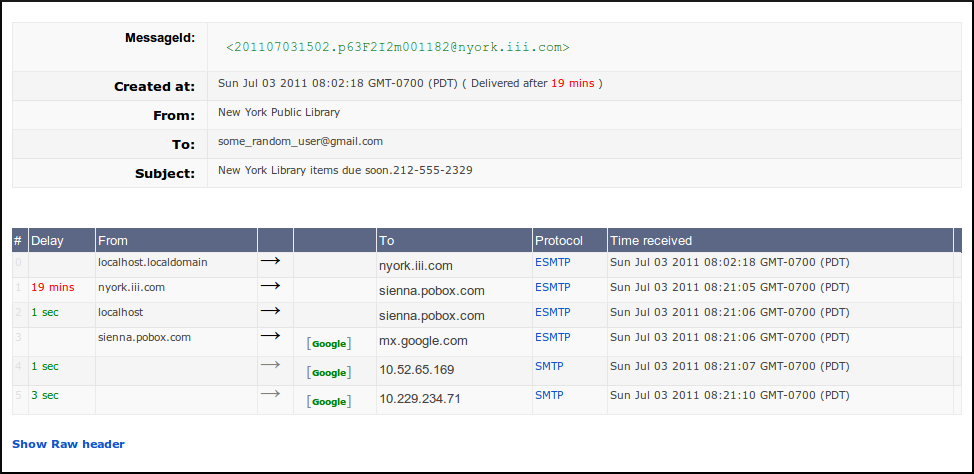
\includegraphics[width=0.9\linewidth]{google-header}\label{fig:goo}
\end{framed}
	\caption{Google Apps Toolbox E-mail header output} \end{figure}

One of the most useful features from the Google Apps Toolbox is the information
provided about the servers the message travelled through.  This tool shows the
details of the time taken for each hop, and the protocol used.

\subsection{Microsoft}

The Microsoft Message Header Analyzer\footnote{Fount at
	\url{https://testconnectivity.microsoft.com/MHA/Pages/mha.aspx}} and
showing sample results in figure~\ref{fig:mic}

\begin{figure}
\begin{framed}
	\centering 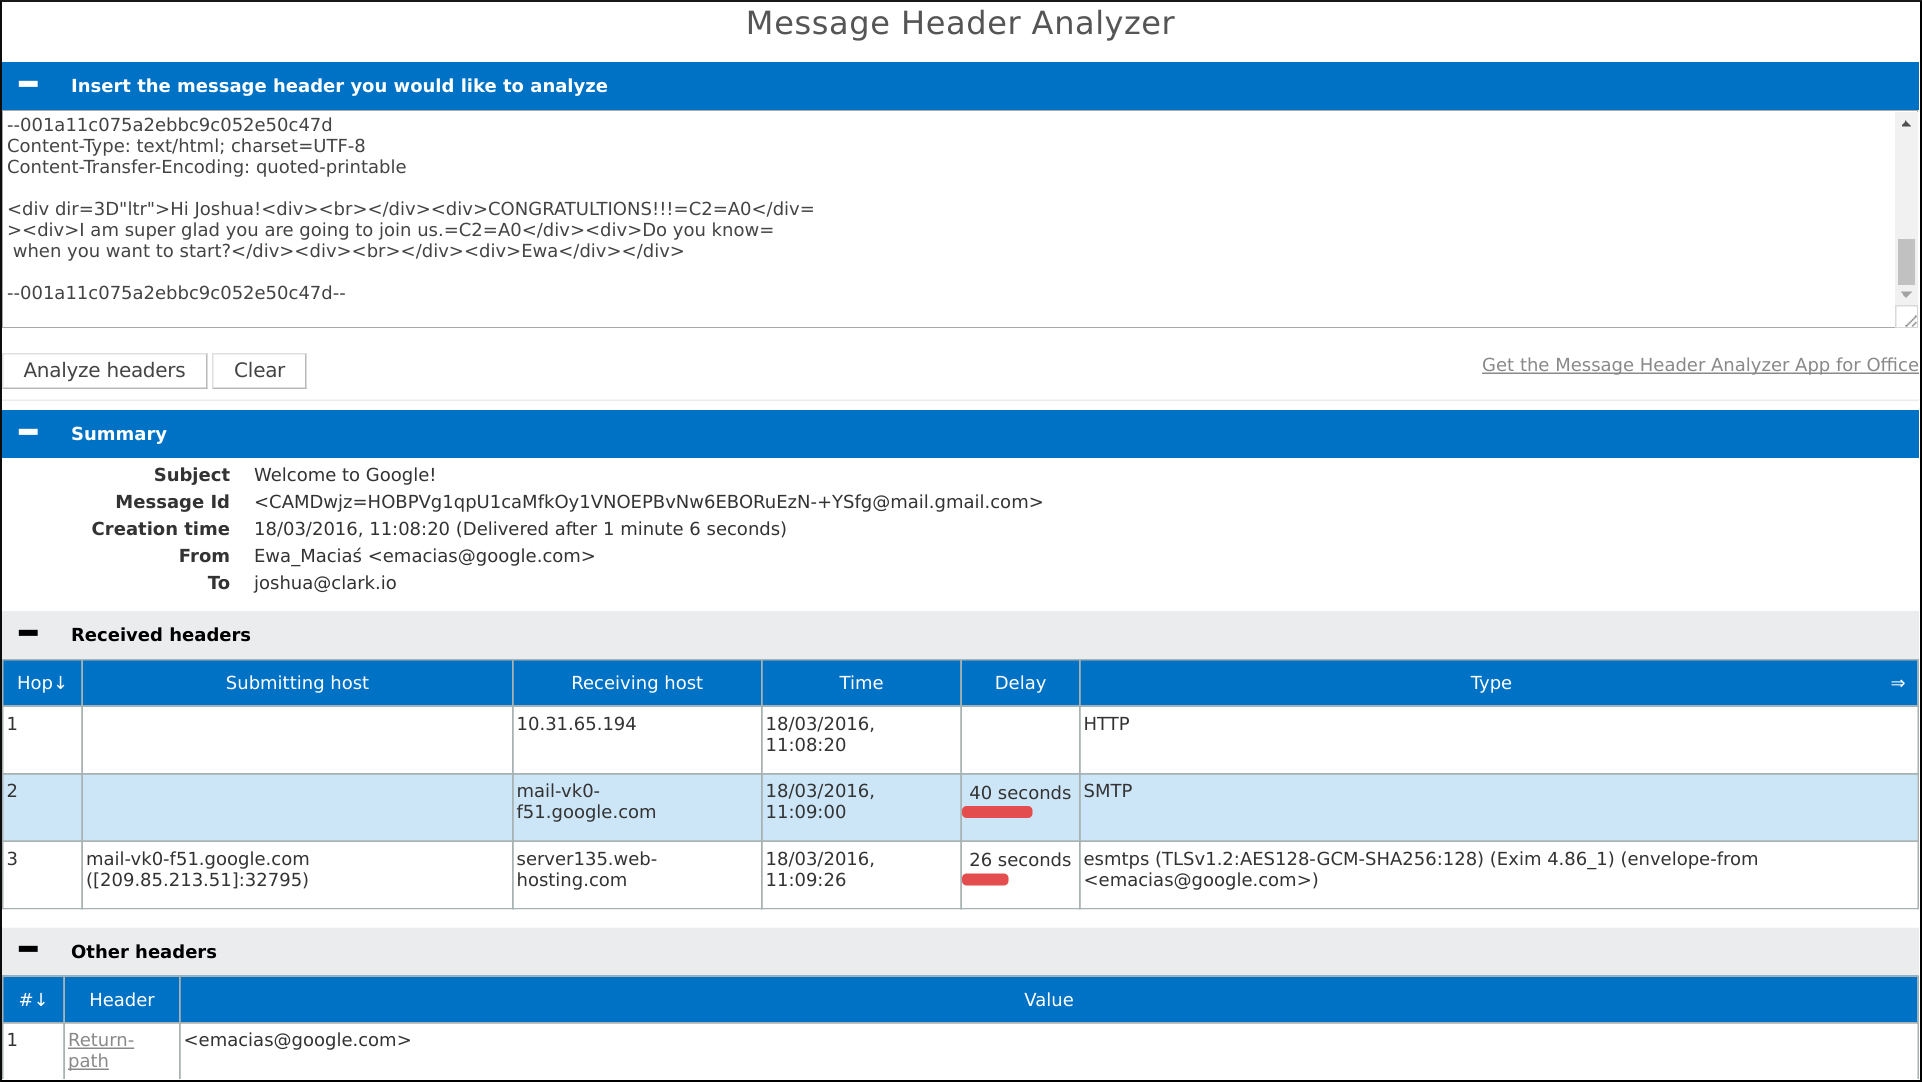
\includegraphics[width=0.9\linewidth]{microsoft-header}\label{fig:mic}
\end{framed}
\caption{Microsoft E-mail header output} \end{figure}

\section{Vulnerabilities}

\epigraph{Beware of bugs in the above code; I have only proved it correct, not tried it.}{Donald Knuth}

Problems in software are nothing new, and seeking to exploit these issues is
almost as old.   As the security implications behind flawed software became more
widely recognised, reducing their impact wherever possible became the next most
important step.  The MITRE Corporation operates the National Cybersecurity
Federally Funded Research and Development Centre, which exists to maintain a
database of these vulnerabilities, which are referred to as Common
Vulnerabilities and Exposures (CVE).

\subsection{CVE Mitre Lookup}

There are a number of tools to look up CVEs\footnote{Fount at
	\url{https://www.cve.mitre.org/find/index.html}} and showing sample
results in figure~\ref{fig:cve}.  There are a number of limitations to the
results returned by the CVE Mitre tool.  Firstly, little context is returned:
information about scores, the impact and access information are omitted, for
example.  Additionally, the process of finding relevant vulnerabilities is
further slowed down by the necessity to search for specific terms one at a
time.  Additionally, automated tools exist at a consumer and enterprise level
that will automatically scan a computer or network to detect installed software
configurations and show the results.

\begin{figure} \begin{framed}\centering 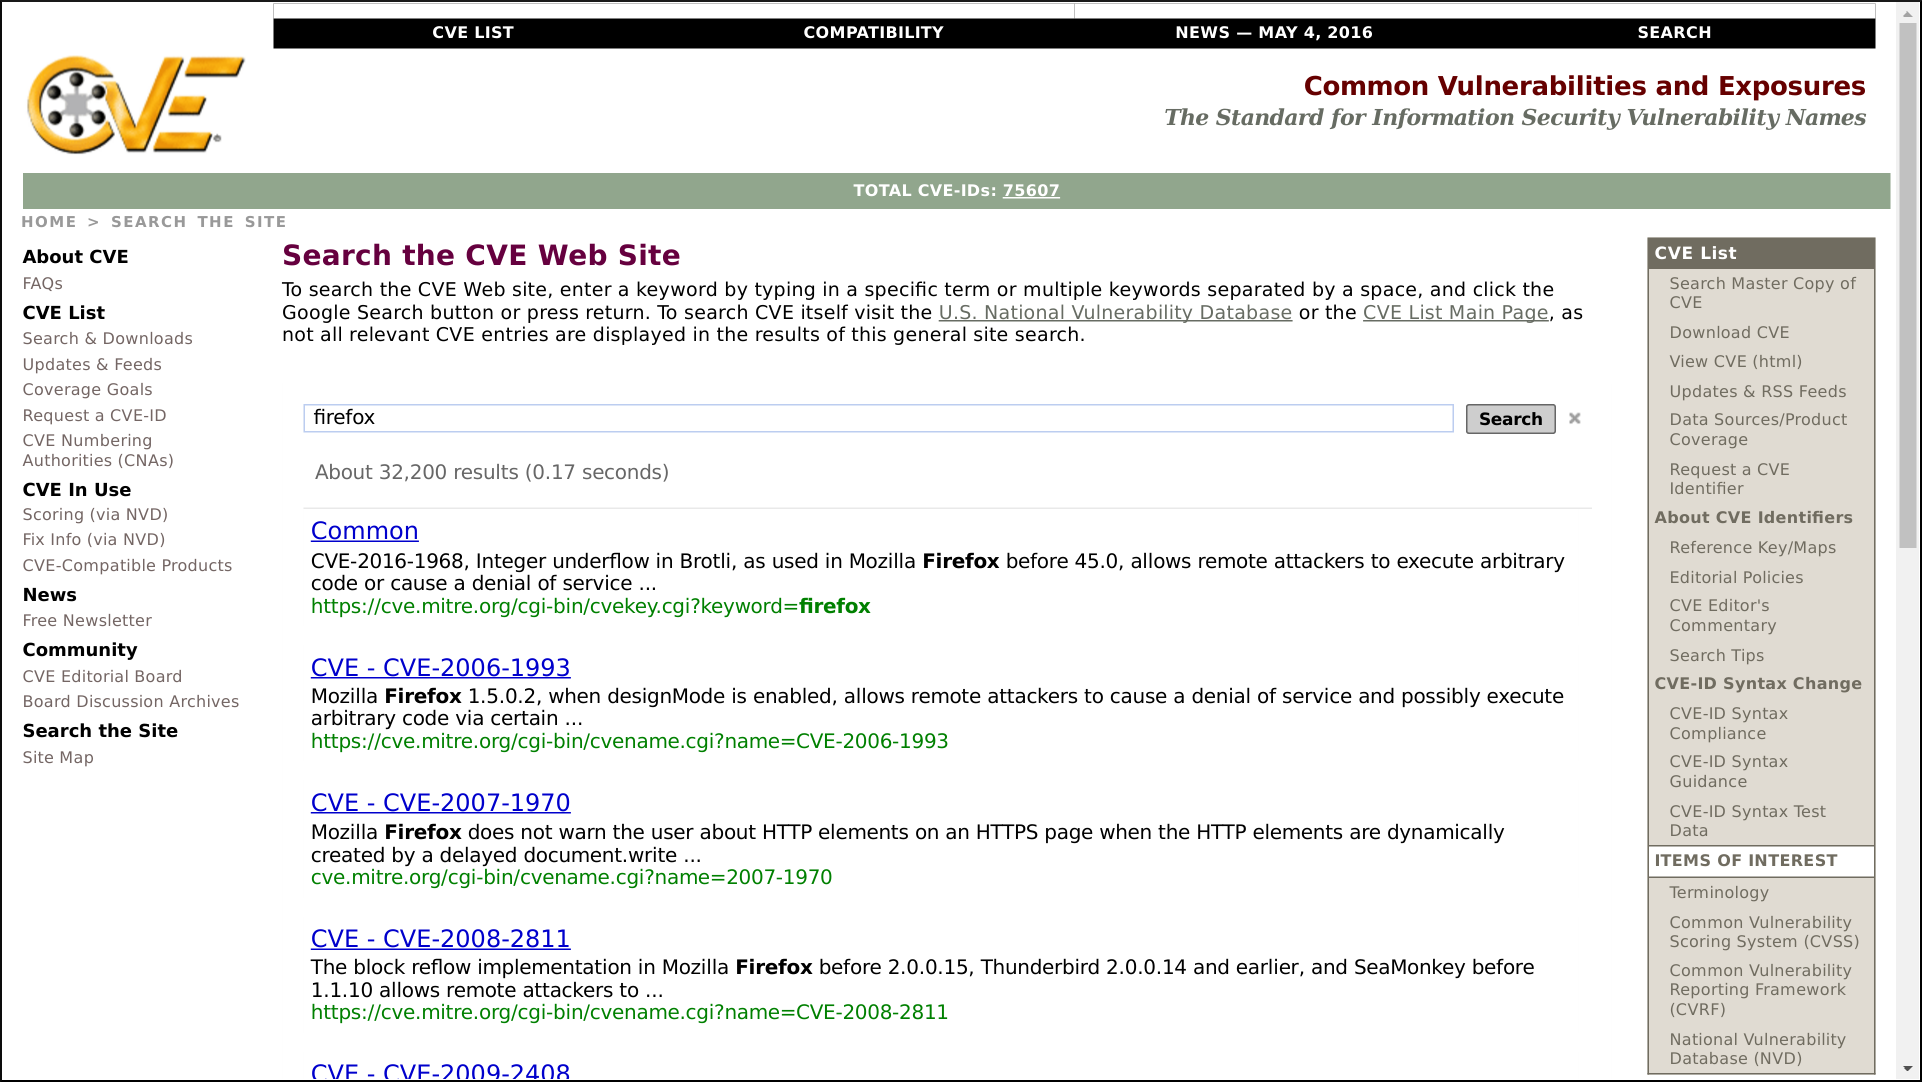
\includegraphics[width=0.9\linewidth]{cve-lookup}\label{fig:cve}\end{framed} \caption{CVE Search Results} \end{figure}

\subsection{Norton Vulnerability Protection}

For example, the now deprecated Norton Vulnerability Protection tool, as shown
in Figure~\ref{fig:nort}\footnote{Available at \url{community.norton.com}}
lists the programs and the total number of  vulnerabilities found, providing
more information on each program.  This method has the advantage of indicating
the specific programs that have vulnerabilities, with the aim of allowing a
user to update their vulnerable applications, however it does not allow for
more fine-grained information.


\begin{figure} \begin{framed} \centering 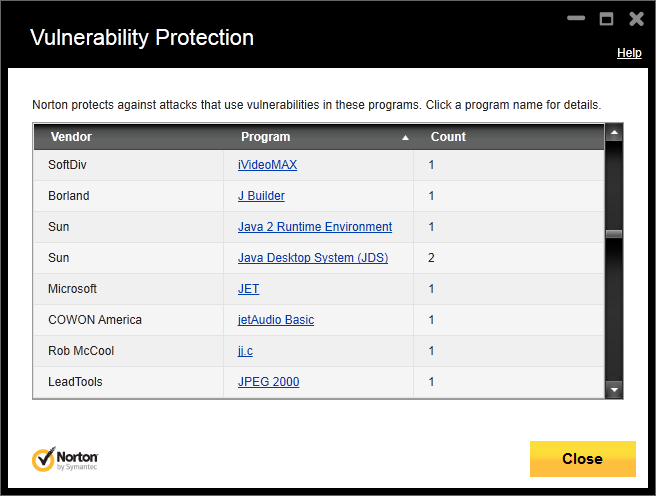
\includegraphics[width=0.9\linewidth]{norton-cve}
\end{framed}
	\label{fig:nort} \caption{Norton Vulnerability Protection Results}
\end{figure}

\section{Overview}
